\section*{Resultados Parciais}
O modelo 2 (figura \ref{fig:pretrained_model}) usa uma rede pré-treinada VGG16 com os pesos da ImageNet. A vantagem de usá-las é que ela tem muitas camadas de convolução e foram treinadas com uma quantidade realmente grande de amostras (da ordem de milhão). Por isso, ela tem muitos filtros para identifcar formas, cores e texturas em imagens.

\pagebreak
\begin{figure}[h!]
  \centering
  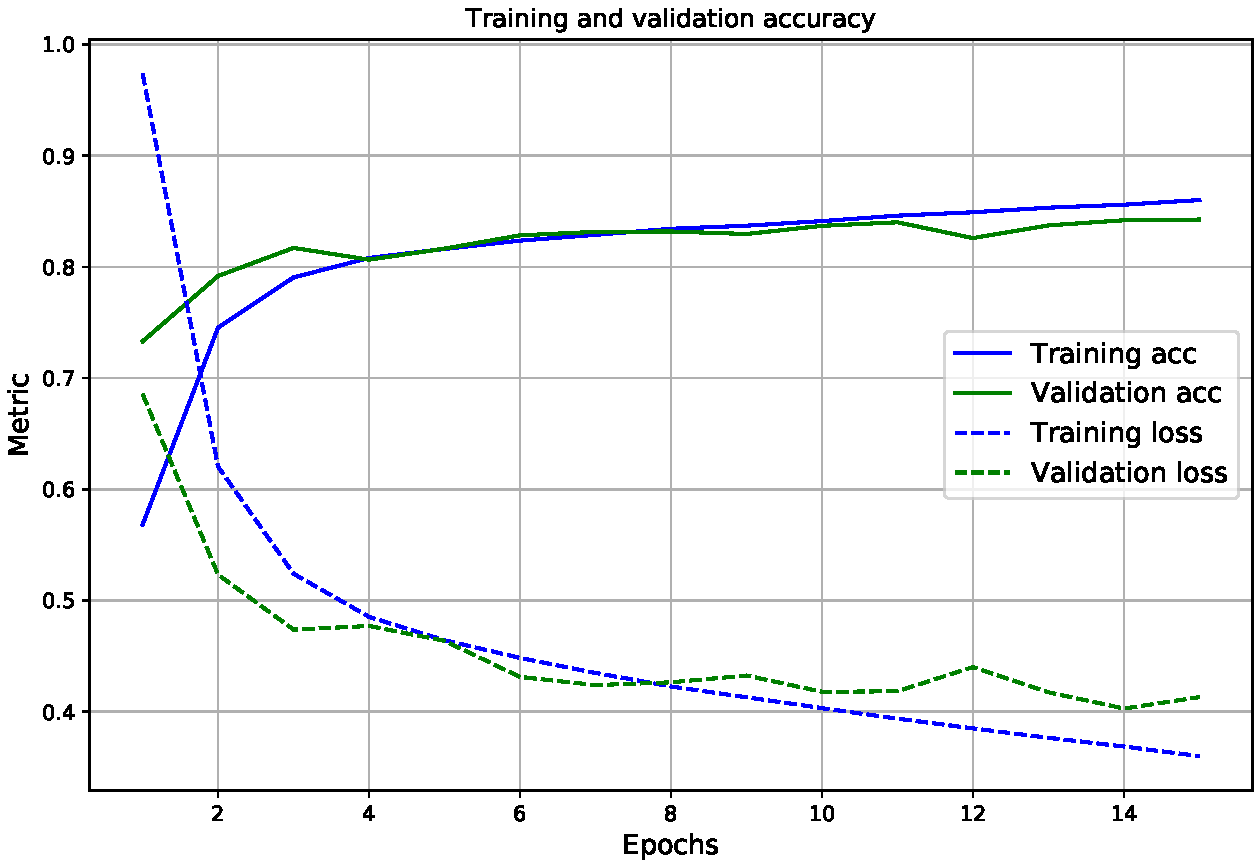
\includegraphics[width=.78\textwidth]{figures/conv_train.pdf}
  \caption{Gráfico da acurácia e perda em cada época de treinamento do modelo 1}
  \label{fig:conv_train}
\end{figure}

\begin{figure}[h!]
  \centering
  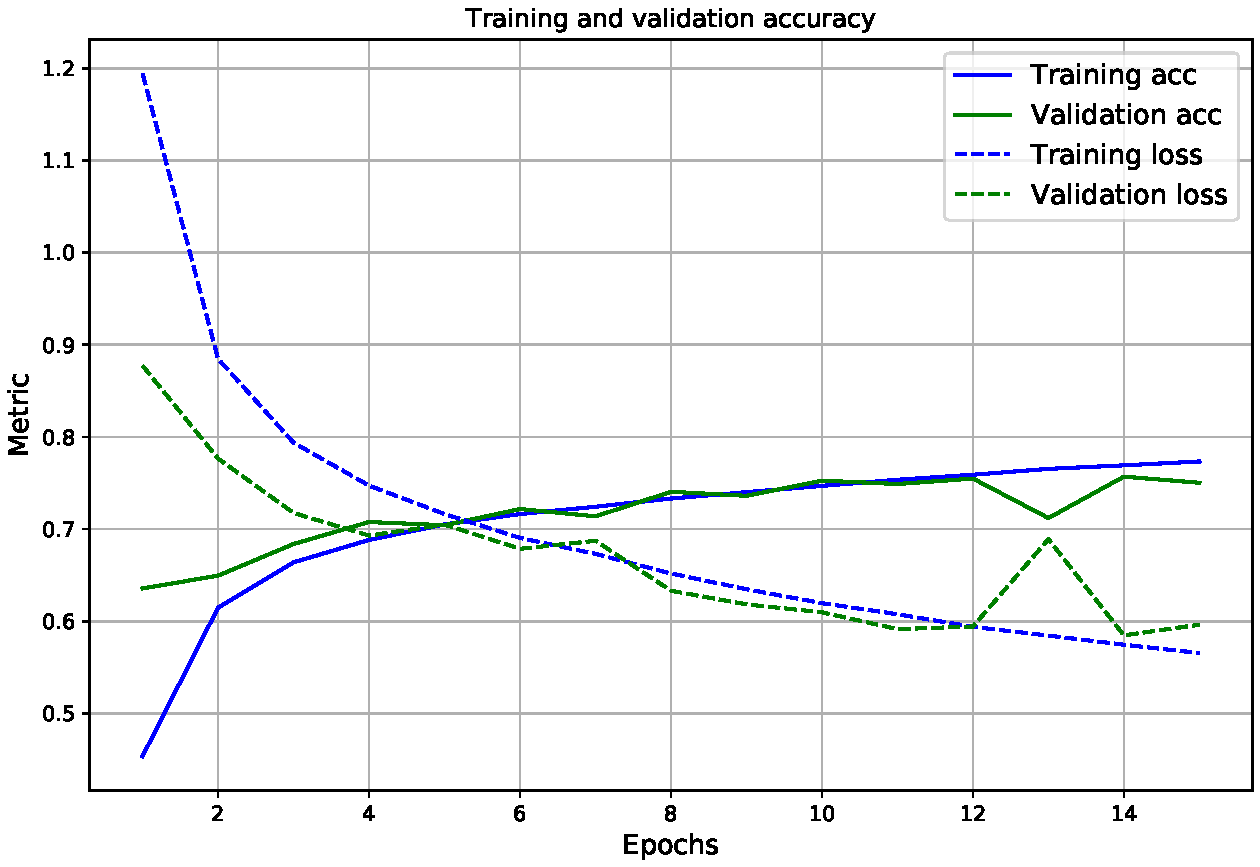
\includegraphics[width=.78\textwidth]{figures/pretrained_train.pdf}
  \caption{Gráfico da acurácia e perda em cada época de treinamento do modelo 2}
  \label{fig:pretrained_train}
\end{figure}